% CONTINUES: exponent of (Z/pqZ)^x, and whether phi(pq)=(p-1)(q-1) is optimal
% --- page 13 ---

If \(p\) and \(q\) are both odd, one can do better. In that case \(p-1\) and \(q-1\) are both even, so \(g=\gcdop(p-1,q-1)\ge 2\) and the exponent below is at most half of \((p-1)(q-1)\).

\begin{keybox}
\begin{theorem}
Let \(p\) and \(q\) be distinct primes, and set \(g=\gcdop(p-1,q-1)\). Then for every integer \(a\) with \(\gcdop(a,pq)=1\),
\[
    a^{(p-1)(q-1)/g}\equiv 1\pmod{pq}.
\]
\end{theorem}
\end{keybox}

\begin{proof}
The quotient \((q-1)/g\) is an integer, and Fermat's little theorem gives \(a^{p-1}\equiv 1\pmod{p}\), so
\[
    a^{(p-1)(q-1)/g}
    =\bigl(a^{p-1}\bigr)^{(q-1)/g}
    \equiv 1\pmod{p}.
\]
The same argument modulo \(q\) yields
\[
    a^{(q-1)(p-1)/g}\equiv 1\pmod{q}.
\]
Thus \(pq\) divides \(a^{(p-1)(q-1)/g}-1\).
\end{proof}

\begin{example}
Take the modulus \(15=3\cdot 5\). Here \(\gcdop(2,4)=2\) and
\[
    \frac{(3-1)(5-1)}{2}=4,
\]
while \(\varphi(15)=8\). The units modulo \(15\) are \(1,2,4,7,8,11,13,14\), and each has fourth power congruent to \(1\):
\begin{align*}
    1^{4}&\equiv 14^{4}\equiv 1,\\
    2^{4}&\equiv 13^{4}\equiv 1,\\
    4^{4}&\equiv 11^{4}\equiv 1,\\
    7^{2}&\equiv 4,\qquad 7^{4}\equiv 8^{4}\equiv 1,
\end{align*}
all modulo \(15\).
% FIX p.13: the notes write a cramped line ``phi(3 x 5) = 8/2 \neq 4''.
% Restored as phi(15)=8 and (p-1)(q-1)/g = 8/2 = 4. The comparison 8 \neq 4 is the point of the example.
In particular
\[
    \gcdop(2,4)=2\implies \varphi(3\cdot 5)=8\neq 4=\frac{8}{2}.
\]
So the exponent \(4\) already works, and it is strictly smaller than \(\varphi(15)\).
\end{example}

Is the exponent \((p-1)(q-1)/g\) optimal?

% --- page 14 ---

Yes. The identity \(\operatorname{lcm}(x,y)=xy/\gcdop(x,y)\) gives
\[
    \frac{(p-1)(q-1)}{g}
    =\frac{(p-1)(q-1)}{\gcdop(p-1,q-1)}
    =\operatorname{lcm}(p-1,q-1).
\]
By the Chinese Remainder Theorem,
\[
    \Z/pq\Z\cong \Z/p\Z\times\Z/q\Z,
\]
and passing to units,
\[
    \units{pq}\cong \units{p}\times\units{q}.
\]

\begin{figure}[H]
\centering
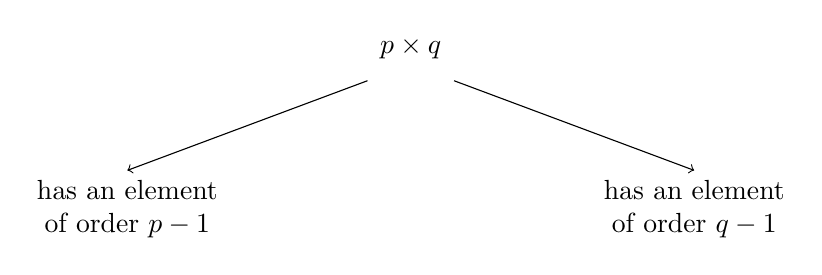
\begin{tikzpicture}
    \node (P) at (0,0.2) {\(\units{p}\times\units{q}\)};
    \node[align=center] (L) at (-3.6,-1.85) {has an element\\ of order \(p-1\)};
    \node[align=center] (R) at ( 3.6,-1.85) {has an element\\ of order \(q-1\)};
    \draw[->] (-0.55,-0.22) -- (L.north);
    \draw[->] ( 0.55,-0.22) -- (R.north);
\end{tikzpicture}
\caption{The two factors of \(\units{pq}\).}
\end{figure}

Each factor is cyclic, so the first has an element of order \(p-1\) and the second an element of order \(q-1\). The corresponding pair in the product then has order \(\operatorname{lcm}(p-1,q-1)\). Hence \(\units{pq}\) has an element of order \(\operatorname{lcm}(p-1,q-1)\), and no smaller positive exponent works for every unit. The exponent in the theorem is optimal.

\begin{remark}
Let \(p\), \(q\), and \(r\) be distinct primes. The largest order of an element of \(\units{pqr}\) is \(\operatorname{lcm}(p-1,q-1,r-1)\). Explicitly, if
\begin{align*}
    a&=\gcdop(p-1,q-1,r-1),&
    b&=\gcdop(p-1,q-1),\\
    c&=\gcdop(q-1,r-1),&
    d&=\gcdop(p-1,r-1),
\end{align*}
then
\[
    \operatorname{lcm}(p-1,q-1,r-1)
    =\frac{(p-1)(q-1)(r-1)\cdot a}{b\cdot c\cdot d}.
\]
\end{remark}

\lectureheading{Lecture 15 (06/10/26)}

Consider the congruence
\[
    x^{e}\equiv c\pmod{N}.
\]
The problem is to find an \(e\)th root of \(c\) modulo \(N\). This is easy when \(N=p\) is prime.

% --- page 15 ---

\begin{proposition}
Let \(p\) be prime and let \(e\ge 1\) satisfy \(\gcdop(e,p-1)=1\). Then the congruence \(x^{e}\equiv c\pmod{p}\) has a unique solution, namely
\[
    x\equiv c^{d}\pmod{p},
\]
where \(ed\equiv 1\pmod{p-1}\).
\end{proposition}

\begin{proof}
If \(c\equiv 0\pmod{p}\), then \(x\equiv 0\pmod{p}\) is a solution. It is the only one: \(p\) divides \(x^{e}\), so \(p\) divides \(x\).

Now assume \(c\not\equiv 0\pmod{p}\), that is \(\gcdop(c,p)=1\). Fermat gives \(c^{p-1}\equiv 1\pmod{p}\). Write \(de=1+k(p-1)\). Then
\begin{align*}
    (c^{d})^{e}
    =c^{de}
    =c^{1+k(p-1)}
    =c\cdot\bigl(c^{p-1}\bigr)^{k}
    \equiv c\cdot 1
    \equiv c\pmod{p}.
\end{align*}
Thus \(x\equiv c^{d}\pmod{p}\) is a solution. If \(x_{1}\) is any other solution, the same congruence \(x_{1}^{p-1}\equiv 1\pmod{p}\) yields
\[
    x_{1}
    \equiv x_{1}^{de}
    =(x_{1}^{e})^{d}
    \equiv c^{d}\pmod{p}.
\]
\end{proof}

\begin{keybox}
\begin{proposition}
Let \(p\) and \(q\) be distinct primes, and let \(e\ge 1\) satisfy \(\gcdop\bigl(e,(p-1)(q-1)\bigr)=1\). Then the congruence \(x^{e}\equiv c\pmod{pq}\) has a unique solution
\[
    x\equiv c^{d}\pmod{pq},
\]
where \(de\equiv 1\pmod{(p-1)(q-1)}\).
\end{proposition}
\end{keybox}

\begin{remark}[Knowing \(p+q\)]
Given \(n=pq\), the value of \(p+q\) determines
\[
    (p-1)(q-1)=pq-(p+q)+1.
\]
Equivalently, \(p\) and \(q\) are the roots of
\[
    (x-p)(x-q)=x^{2}-(p+q)x+pq.
\]
\end{remark}

\begin{remark}
It is not yet clear whether \(x^{e}\equiv c\pmod{pq}\) can be solved without computing \(\varphi(pq)=(p-1)(q-1)\).
\end{remark}

% --- page 16 ---

\begin{proof}
Write \(de=1+t(p-1)(q-1)\).

If \(c\equiv 0\pmod{pq}\), then \(x\equiv 0\pmod{pq}\) is a solution.

Suppose next that \(\gcdop(c,pq)=p\), and write \(c=ps\) with \(\gcdop(s,q)=1\). Both \(c^{de}\) and \(c\) are divisible by \(p\), so \(c^{de}\equiv c\pmod{p}\). Modulo \(q\), Fermat applies to \(ps\) because \(\gcdop(ps,q)=1\):
\begin{align*}
    c^{de}
    &=(ps)^{1+t(p-1)(q-1)}
     =ps\cdot\bigl((ps)^{q-1}\bigr)^{t(p-1)}\\
    &\equiv ps\cdot 1
     \equiv c\pmod{q}.
\end{align*}
% FIX p.16: the reduction modulo \(q\) is written \((pk)^{1+t(p-1)(q-1)}\equiv (pk)'\equiv c\pmod{q}\). The mark after \((pk)\) is a shorthand for the Fermat reduction \((pk)^{q-1}\equiv 1\pmod{q}\), which is the step displayed above.
Thus \(c^{de}\equiv c\pmod{pq}\). The case \(\gcdop(c,pq)=q\) is symmetric.

If instead \(\gcdop(c,pq)=1\), Euler's theorem gives \(c^{(p-1)(q-1)}\equiv 1\pmod{pq}\), and
\[
    (c^{d})^{e}
    =c^{de}
    =c^{1+t(p-1)(q-1)}
    \equiv c\pmod{pq}.
\]
In every case, \(x\equiv c^{d}\pmod{pq}\) is a solution.

For uniqueness, reduce modulo \(p\) and modulo \(q\). The hypothesis \(\gcdop\bigl(e,(p-1)(q-1)\bigr)=1\) implies \(\gcdop(e,p-1)=\gcdop(e,q-1)=1\), and \(de\equiv 1\) modulo both \(p-1\) and \(q-1\). The previous proposition supplies a unique solution modulo \(p\) and a unique solution modulo \(q\), so the Chinese Remainder Theorem supplies a unique solution modulo \(pq\).
% The notes spell out existence in the three cases above. The uniqueness sentence
% is the same reduction, which the proposition claims and the prime case already contains.
\end{proof}

\begin{remark}
The exponent \(d\) can be obtained by solving
\[
    de\equiv 1\pmod{\frac{(p-1)(q-1)}{g}},
    \qquad g=\gcdop(p-1,q-1),
\]
rather than modulo \((p-1)(q-1)\). The modulus here is \(\operatorname{lcm}(p-1,q-1)\).
\end{remark}

\subsection{The process}
% The page ends mid-parenthesis at ``(let n''. Completed as n=pq.
\begin{keybox}[title=The RSA cryptosystem]
Alice proceeds as follows.
\begin{enumerate}[leftmargin=1.6em]
    \item Choose two distinct primes \(p\) and \(q\). The primes are taken close to each other, for security reasons. Set \(n=pq\). (Lectures~17 and~18 make this precise: \(p\) and \(q\) should have similar size, but must not be so close that Fermat's difference-of-squares method finds them.)
    \item Choose an integer \(e\) with \(1<e<\varphi(n)\) and \(\gcdop\bigl(e,\varphi(n)\bigr)=1\). This \(e\) is the encryption exponent.
\end{enumerate}

% --- page 17 ---

\begin{enumerate}[leftmargin=1.6em, resume]
    \item Publish \(n\) and \(e\).
    \item Bob takes a message \(m\), computes \(c\equiv m^{e}\pmod{n}\), and sends \(c\) to Alice.
    \item Alice must solve \(x^{e}\equiv c\pmod{n}\). She recovers
    \[
        m\equiv c^{d}\pmod{n},
    \]
    where \(de\equiv 1\pmod{(p-1)(q-1)}\).
\end{enumerate}
\end{keybox}

\subsection{Choosing the encryption exponent}
Often \(e=3\) works. Writing the exponent as one more than a power of two makes the power cheap:
\begin{align*}
    3&=2+1, & m^{3}&=m^{2}\cdot m,\\
    m^{5}&=(m^{2})^{2}\cdot m, &
    m^{9}&=\bigl((m^{2})^{2}\bigr)^{2}\cdot m.
\end{align*}
In general, if \(e=2^{k}+1\), then \(m^{e}\) is \(k\) squarings followed by one multiplication. The usual choice is the Fermat prime
\[
    e=2^{16}+1=65537=2^{2^{4}}+1=F_{4},
\]
where \(F_{r}=2^{2^{r}}+1\) is the \(r\)th Fermat number.

\begin{example}
Take \(p=71\) and \(q=89\), so \(n=6319\). Then
\[
    \varphi(n)=70\cdot 88=6160.
\]
The exponent \(e=53\) has inverse \(d=2557\) modulo \(6160\). For the message \(m=2161\),
\[
    c\equiv m^{e}\equiv 3248\pmod{6319},
\]
and \(3248^{2557}\equiv 2161\pmod{6319}\).
\end{example}

% --- page 18 ---

\section{Primality and factorization}
% ============================================================

Fermat's little theorem says that \(a^{p}\equiv a\pmod{p}\) for every integer \(a\) and every prime \(p\). The same congruence can hold when the modulus is composite. For instance
\[
    2^{341}\equiv 2\pmod{341},
\]
but \(341=11\cdot 31\).

The contrapositive is a primality test. If \(n\) is a positive integer and \(a\) is an integer with \(a^{n}\not\equiv a\pmod{n}\), then \(n\) is not prime.

\begin{definition}
Let \(n>1\). An integer \(a\) is a \emph{witness of compositeness} of \(n\) if
\[
    a^{n}\not\equiv a\pmod{n}.
\]
\end{definition}

For example, modulo \(6\),
\begin{align*}
    2^{2}&\equiv 4, &
    2^{4}&\equiv 4, &
    2^{6}&\equiv 4\not\equiv 2\pmod{6}.
\end{align*}
Hence \(2\) is a witness of compositeness of \(6\).

If \(n\) is composite, must some witness exist? Unfortunately, no. One has
\[
    a^{561}\equiv a\pmod{561}
\]
for every integer \(a\), while \(3\) divides \(561\), so \(561\) is not prime. Such moduli are the Carmichael numbers.

% --- page 19 ---

There are in fact infinitely many Carmichael numbers: the set \(\{n:1<n\le x\}\) contains at least \(x^{1/3}\) Carmichael numbers as \(x\to\infty\).

\begin{definition}
A composite positive integer \(n\) is a \emph{Carmichael number} if
\[
    a^{n}\equiv a\pmod{n}
    \qquad\text{for every }a\in\Z.
\]
\end{definition}

This forces a different primality test.

\subsection{The Miller--Rabin test}

\begin{keybox}
\begin{proposition}
Let \(p\) be an odd prime, and write \(p-1=2^{k}q\) with \(q\) odd. Let \(a\) be an integer with \(\gcdop(a,p)=1\). Then one of the following holds.
\begin{enumerate}[label=\textup{(\roman*)}, leftmargin=1.6em]
    \item \(a^{q}\equiv 1\pmod{p}\).
    \item At least one of
    \(a^{q},\, a^{2q},\, a^{2^{2}q},\, \ldots,\, a^{2^{k-1}q}\)
    is congruent to \(-1\) modulo \(p\).
\end{enumerate}
\end{proposition}
\end{keybox}

\begin{proof}
If \(a^{q}\equiv 1\pmod{p}\), there is nothing to prove. Suppose otherwise, and consider the list
\[
    a^{q},\; a^{2q},\; \ldots,\; a^{2^{k-1}q}.
\]
At least one entry is not congruent to \(1\) modulo \(p\). On the other hand Fermat gives
\[
    a^{2^{k}q}=a^{p-1}\equiv 1\pmod{p}.
\]
The congruence \(x^{2}\equiv 1\pmod{p}\) has exactly two solutions, namely \(x\equiv 1\pmod{p}\) and \(x\equiv -1\pmod{p}\). Let \(j\ge 1\) be minimal such that \(a^{2^{j}q}\equiv 1\pmod{p}\). Then
\[
    \bigl(a^{2^{j-1}q}\bigr)^{2}\equiv 1\pmod{p}
\]
and \(a^{2^{j-1}q}\not\equiv 1\pmod{p}\), so \(a^{2^{j-1}q}\equiv -1\pmod{p}\).
% The notes stop once the two roots of x^2 \equiv 1 are named; the choice of j is the missing sentence.
\end{proof}

% --- page 20 ---

\begin{definition}
Let \(n\) be odd, and write \(n-1=2^{k}q\) with \(q\) odd. An integer \(a\) with \(\gcdop(a,n)=1\) is a \emph{Miller--Rabin witness} for the compositeness of \(n\) if both of the following hold.
\begin{enumerate}[label=\textup{(\roman*)}, leftmargin=1.6em]
    \item \(a^{q}\not\equiv 1\pmod{n}\).
    \item \(a^{2^{i}q}\not\equiv -1\pmod{n}\) for every \(0\le i<k\).
\end{enumerate}
If such an \(a\) exists, then \(n\) is composite.
\end{definition}

\begin{example}
Factor \(561=3\cdot 11\cdot 17\), so \(560=2^{4}\cdot 35\). The powers to check for the base \(2\) are \(2^{35}\), \(2^{70}\), \(2^{140}\), and \(2^{280}\). Their residues modulo \(561\) are
\begin{align*}
    2^{35}&\equiv 263, &
    2^{70}&\equiv 166, &
    2^{140}&\equiv 67, &
    2^{280}&\equiv 1.
\end{align*}
None of these is congruent to \(-1\), and \(2^{35}\not\equiv 1\), so \(2\) is a Miller--Rabin witness for \(561\).
% The notes list the four powers and say ``check'', without writing the residues.
\end{example}

How likely is the test to succeed? If \(n>1\) is an odd composite number, at most one quarter of the integers \(a\) with \(1\le a\le n-1\) are strong liars, meaning \(a^{q}\equiv 1\pmod{n}\) or \(a^{2^{i}q}\equiv -1\pmod{n}\) for some \(0\le i<k\). Every other such \(a\) proves that \(n\) is composite: either \(\gcdop(a,n)>1\), or \(a\) is a Miller--Rabin witness. The test therefore succeeds for at least \(75\%\) of these bases.
% FIX p.20: the notes say that at least \(75\%\) of the \(a\) in \(1,\ldots,n-1\) are Miller--Rabin witnesses. A witness, as defined above, has to be coprime to \(n\), and that stronger count is false. For \(n=561\) only \(310\) of the \(560\) residues are witnesses, while \(240\) share a factor with \(561\). Rabin's theorem bounds the strong liars by \((n-1)/4\), so the \(75\%\) includes the bases with \(\gcdop(a,n)>1\).

\subsection{The prime number theorem}

Let \(x\) be a positive real number, and let
\[
    \pi(x)=\#\{n\le x:n\text{ is prime}\}.
\]
Gauss conjectured the asymptotic below. It was proved by Hadamard and de la Vall\'ee Poussin.
% FIX p.20: the notes spell the second name ``de la vavee Poussin''.

\begin{theorem}[Prime number theorem]
\[
    \lim_{x\to\infty}\frac{\pi(x)}{x/\log x}=1.
\]
Equivalently, the \(n\)th prime satisfies \(p_{n}\sim n\log n\).
\end{theorem}

% --- page 21 ---

\lectureheading{Lecture 16 (09/10/26)}

\section{The Miller--Rabin test, revisited}
% ============================================================

The two facts used to run the test are restated as follows.

\begin{theorem}
Let \(p\) be an odd prime, and write \(p-1=2^{k}q\) with \(q\) odd. Let \(a\) be an integer not divisible by \(p\). Then one of the following holds.
\begin{enumerate}[label=\textup{(\roman*)}, leftmargin=1.6em]
    \item \(a^{q}\equiv 1\pmod{p}\).
    \item One of \(a^{q},\, a^{2q},\, a^{2^{2}q},\, \ldots,\, a^{2^{k-1}q}\) is congruent to \(-1\) modulo \(p\).
\end{enumerate}
\end{theorem}

\begin{theorem}
If \(n\) is an odd composite, then at least \(75\%\) of the integers \(a\) with \(1\le a\le n-1\) prove that \(n\) is composite, either because \(\gcdop(a,n)>1\) or because \(a\) is a Miller--Rabin witness.
\end{theorem}

Thus if \(n\) is composite, a search can fail. In the worst case one may have to go through \(n/4\) bases that do not prove compositeness before finding one that does.
% FIX p.21: same correction as on page~20. The scan says ``between \(1\) and \(n\)''; the count is over \(1\le a\le n-1\), and \(n\) itself is excluded. The hypothesis is that \(n\) is odd, since \(n-1=2^{k}q\) is the setup of the test.

Eric Bach's theorem says that, under the generalized Riemann hypothesis, a composite \(n\) has a Miller--Rabin witness
\[
    a\le \bigl[2(\log n)^{2}\bigr].
\]
The result is conjectural, in the sense that it depends on an unproved hypothesis.

\subsection{The AKS primality test}
Can one test primality in time polynomial in \(\log n\), with no unproved hypothesis? In \(2002\), Agrawal, Kayal, and Saxena gave such a test (AKS).
% FIX p.21: the notes spell the first name ``Agarwal''.

Recall that \(a^{p}\equiv a\pmod{p}\) for every prime \(p\) and every integer \(a\). The converse fails: \(a^{n}\equiv a\pmod{n}\) does not imply that \(n\) is prime.

% --- page 22 ---

\begin{lemma}[AKS]
Let \(\gcdop(a,n)=1\) and \(n\ge 2\). Then \(n\) is prime if and only if
\[
    (x+a)^{n}\equiv x^{n}+a\pmod{n}
\]
in \((\Z/n\Z)[x]\).
\end{lemma}

\begin{proof}
Suppose \(n\) is prime. The binomial theorem, or the freshman's dream, gives \((x+a)^{n}\equiv x^{n}+a^{n}\pmod{n}\), because \(n\) divides \(\binom{n}{k}\) for \(0<k<n\). Fermat's little theorem gives \(a^{n}\equiv a\pmod{n}\), and the two congruences combine.

Conversely, suppose \((x+a)^{n}\equiv x^{n}+a\pmod{n}\). Expanding and comparing coefficients, \(n\) divides \(\binom{n}{k}a^{k}\) for every \(1\le k\le n-1\). Since \(\gcdop(a,n)=1\), it follows that \(n\) divides \(\binom{n}{k}\) for every such \(k\).

Suppose \(n\) is composite, and let \(p\) be a prime divisor of \(n\). Then
\[
    \binom{n}{p}
    =\frac{n(n-1)\cdots(n-p+1)}{p!}
    =\frac{n}{p}\binom{n-1}{p-1}.
\]
% The notes cross out a truncated form of this identity, n/p times (n-1)/(p-1).
Since \(n\) divides \(\binom{n}{p}\), one has \(\binom{n}{p}=nt\) for some integer \(t\), and cancelling \(n/p\) yields
\[
    \binom{n-1}{p-1}=pt.
\]
Thus \(p\) divides \(\binom{n-1}{p-1}\). Writing
\[
    \binom{n-1}{p-1}
    =\frac{(n-1)(n-2)\cdots(n-p+1)}{(p-1)!}
\]
and using that \(p\) does not divide \((p-1)!\), one concludes that \(p\) divides \({(n-1)\cdots(n-p+1)}\). But \(p\) divides \(n\), so \(p\) divides none of the integers \(m\) with \(n-p<m<n\). Those integers are precisely the factors \(n-1,\ldots,n-p+1\), a contradiction.
\end{proof}

% --- page 23 ---

\begin{remark}
The lemma is a primality test, but it is not effective: it asks for a congruence of polynomials of degree \(n\).
\end{remark}

The idea of AKS is to group the binomial coefficients, and to check the grouped sums instead of the individual ones. Set
\[
    f_{a}(x)=(x+a)^{n}-x^{n}-a=\sum_{k=0}^{n-1}b_{k}x^{k}.
\]
% FIX p.23: the notes write (x+a)^n - x^n + a. The polynomial that the lemma
% sets to 0 is (x+a)^n - x^n - a. The degree is at most n-1 because the x^n terms cancel.
Read this polynomial modulo \(x^{r}-1\), for a suitable integer \(r\). In that quotient one has \(x^{r}\equiv 1\), hence \(x^{r+1}\equiv x\) and
\[
    x^{r+r}=x^{2r}\equiv x^{r}\equiv 1.
\]
Therefore \(x^{m}\equiv x^{m\bmod r}\) modulo \(x^{r}-1\), and
\[
    \sum_{k=0}^{n-1}b_{k}x^{k}
    \equiv\sum_{0\le c<r}h_{a}(c)\,x^{c}
    \pmod{x^{r}-1},
\]
where
\[
    h_{a}(c)
    =\sum_{\substack{0\le k\le n-1\\ k\equiv c\pmod{r}}}b_{k}.
\]
If \(h_{a}(c)\not\equiv 0\pmod{n}\) for some such \(r\) and \(c\), then \(n\) is composite.

\begin{keybox}
\begin{theorem}[AKS]
The following algorithm decides whether \(n\) is prime in time polynomial in \(\log n\).
\begin{enumerate}[leftmargin=1.6em]
    \item Check whether \(n\) is a perfect power, that is, whether \(n=a^{b}\) for integers \(a,b>1\). If so, \(n\) is composite.
% --- page 24 ---
    \item Find the minimal integer \(r\) with \(\gcdop(r,n)=1\) and
    \[
        \ord_{r}(n)>(\log n)^{2},
    \]
    where \(\ord_{r}(n)\) is the multiplicative order of \(n\) modulo \(r\). The lower bound on the order is what keeps the algorithm from declaring a composite to be prime.
    \item For \(2\le a\le r\), if \(1<\gcdop(a,n)<n\), then \(n\) is composite.
    \item If \(r\ge n\), then \(n\) is prime.
    \item If \(r<n\), then for each
    \[
        1\le a\le\bigl\lfloor\sqrt{\varphi(r)}\,\log n\bigr\rfloor
        \quad\text{and}\quad
        0\le c\le r,
    \]
    check whether \(h_{a}(c)\equiv 0\pmod{n}\). If some value is nonzero, \(n\) is composite. If every value is zero, \(n\) is prime, and the algorithm stops.
\end{enumerate}
% UNCLEAR p.24: the range on c is written ``0 \le c \le r''. Reducing modulo x^r-1
% only produces coefficients for 0 \le c < r; the endpoint c=r repeats c=0.
\end{theorem}
\end{keybox}

\subsection{Running time}
For the perfect-power test one tries exponents \(b\) in the range \(2\le b\le L\), where \(L=\log_{2} n\), and for each \(b\) one looks for a base \(a\).

\begin{figure}[H]
\centering
\begin{tikzpicture}
    \draw (0,0) -- (6.2,0);
    \draw (0,-0.12) -- (0,0.12);
    \draw (6.2,-0.12) -- (6.2,0.12);
    \node[below] at (3.1,-0.15) {\(1<a<n\)};
\end{tikzpicture}
\caption{The integer \(a\), if it exists, lies strictly between \(1\) and \(n\).}
\end{figure}

\noindent
A candidate \(a\) can be tested with \(O(\log n)\) attempts, by a binary search for the integer \(b\)th root. Hence step~1 runs in \(O\bigl((\log n)^{*}\bigr)\) operations.
% UNCLEAR p.24: the exponent in this big-O bound is written as a star, not a specific integer.

The AKS analysis shows that an integer \(r\) satisfying the order condition can be found in \(\ll(\log n)^{5}\) steps, so step~2 runs in polynomial time. Together these bounds ensure that the algorithm ends in polynomial time.

For RSA, what one needs is factorization.
